\chapter{実験と考察}
本章では、実験の流れについて説明していく。

\section{目的}
本研究の目的は、word2vecの出力ベクトルを利用して語の相似関係を抽出することであり、この実験では、一対の単語ペアを入力とし、入力単語それぞれの近傍n個ずつの単語で作った二つのグループに梅山氏の提案手法を用いることでグループ内の単語同士の対応関係を出力する。

\section{実験データ}
用いた実験データについて説明する。

コーパスとして用いたのは、2016年9月時点での日本語版Wikipedia最新記事\footnote{https://dumps.wikimedia.org/jawiki/20160901/jawiki-20160901-pages-articles.xml.bz2}であり、ここからテキストデータを抽出し、MeCabを用いて形態素毎に分かち書きした。

次に、word2vecを用いて分かち書きしたコーパスから形態素の意味表現ベクトルを学習した。ベクトル学習のハイパーパラメータは以下の通りである。
\begin{itemize}
  \item 適用手法:CBoW
  \item 学習するベクトルの次元数:200
  \item 文脈窓:8
  \item ネガティブサンプリング:
  \item 階層型ソフトマックス:
\end{itemize}
文脈窓は、学習する際に使用する、対象語の前後の文脈語数で、今回文脈語は全部で16個使っている。

\section{梅山氏の手法の有効性確認}
まず初めに、word2vecの出力ベクトルデータを元に、単語同士の相似関係を梅山氏のグラフノードマッチング手法を利用して抽出できるかどうかを確認した。
\subsubsection{用いた単語群}
\begin{table}[h]
  \begin{minipage}[t]{.45\textwidth}
    \caption[テストデータ]{手法の妥当性確認のためのテストデータ}
    \label{test_pre}
    \begin{center}
      \begin{tabular}{|c||c|} \hline
        集合X & 集合Y \\ \hline \hline
        叔父 & 妹 \\
        王 & 祖母 \\
        老人 & 王女 \\
        父 & 雌 \\
        兄 & 老婆 \\
        祖父 & 花子 \\
        弟 & 姉 \\
        息子 & 叔母 \\
        雄 & 娘 \\
        太郎 & 母 \\ \hline
      \end{tabular}
    \end{center}
  \end{minipage}
  \hfill
  \begin{minipage}[t]{.45\textwidth}
    \caption[テストデータのノードマッチング解析結果]{テストデータのノードマッチング解析結果}
    \label{test_bfr}
    \begin{center}
      \begin{tabular}{|c||c|} \hline
        集合X & 集合Y \\ \hline \hline
        叔父 & 叔母 \\
        王 & 王女 \\
        老人 & 老婆 \\
        父 & 母 \\
        兄 & 姉 \\
        祖父 & 祖母 \\
        弟 & 妹 \\
        息子 & 娘 \\
        雄 & 雌 \\
        太郎 & 花子 \\ \hline
      \end{tabular}
    \end{center}
  \end{minipage}
\end{table}
男という括りにできる単語グループXと、女という括りにできるグループYを、それぞれ対になる単語が含まれるように作成した(例:父-母、雄-雌)表(\ref{test_pre})である。もう一方の表(\ref{test_bfr})は、ノードマッチングを適用した結果である。

\subsection{ベクトル行列の作成}
word2vecが出力した各単語のベクトルを、それぞれ行ベクトル$x_i\in X$、$y_i\in Y$とすると、$U_X$、$U_Y$は以下のように表せる。
\begin{equation}
  U_X=\begin{pmatrix}
    x_1 \\
    \vdots \\
    x_n
  \end{pmatrix} \notag \\
  U_Y=\begin{pmatrix}
    y_1 \\
    \vdots \\
    y_n
  \end{pmatrix} \notag \\
\end{equation}
$U_X$、$U_Y$はそれぞれ、第\ref{s_ts}節で述べた$U_G$、$U_H$に対応する。

グループXの単語と、グループYの単語は、それぞれのグループにおいて、重み付きグラフを重みを二点間の距離に反映してベクトル空間上に埋め込んだものとみて、$U_G$、$U_H$の代わりに$U_X$、$U_Y$を用いて、梅山氏の提案手法を適用した。

グループX、Yに関して、梅山氏の提案手法によるノードマッチングを適用した結果が表(\ref{test_bfr})の通りであるから、ある括りで作られた単語グループ同士では、ほぼ同型のグラフ構造が得られ、梅山氏のノードマッチングの適用で対応する単語同士を発見できることと、word2vecの出力ベクトルは単語の相似関係を保持できていることが予想できる。

\subsection{着目形態素の近傍形態素の様子}
次に、入力された単語対それぞれの近傍単語から取得した単語で作成したグループ同士にノードマッチングを適用することで、単語同士の掃除関係が抽出できるかを実験した。

この実験を始めるにあたって、まず、近傍単語の様子を確認した。

\begin{table}[h]
  \begin{minipage}[t]{.45\textwidth}
    \caption[(王,女王)]{(王,女王)の近傍単語}
    \label{kq_table}
    \begin{center}
      \begin{tabular}{|c|c|} \hline
        王 & 女王 \\ \hline
        は王 & 王女 \\
        皇帝 & 王妃 \\
        に王 & 国王 \\
        国王 & エリザベス女王 \\
        君主 & ヴィクトリア \\
        大王 & 王 \\
        王妃 & 王子 \\
        伯 & エリザベス1世 \\
        聖王 & エリザベス2世 \\
        女王 & 王配 \\ \hline
      \end{tabular}
    \end{center}
  \end{minipage}
  \hfill
  \begin{minipage}[t]{.45\textwidth}
    \caption[(日本,アメリカ)]{(日本,アメリカ)の近傍単語}
    \begin{center}
      \begin{tabular}{|c|c|} \hline
        日本 & アメリカ \\ \hline
        韓国 & 米国 \\
        日本国内 & イギリス \\
        台湾 & 英国 \\
        中国 & カナダ \\
        欧米 & アメリカ合衆国 \\
        海外 & ヨーロッパ \\
        日本の文化 & オーストラリア \\
        日本国外 & フランス \\
        アジア & ドイツ \\
        わが国 & キューバ \\ \hline
      \end{tabular}
    \end{center}
  \end{minipage}
\end{table}

\newpage

表(\ref{kq_table})に関して、下図にあるような、(男,女)の関係に相当する単語が出力されることを想定していたため、この時点では大きな誤算である。
\begin{figure}[h]
  \centering
  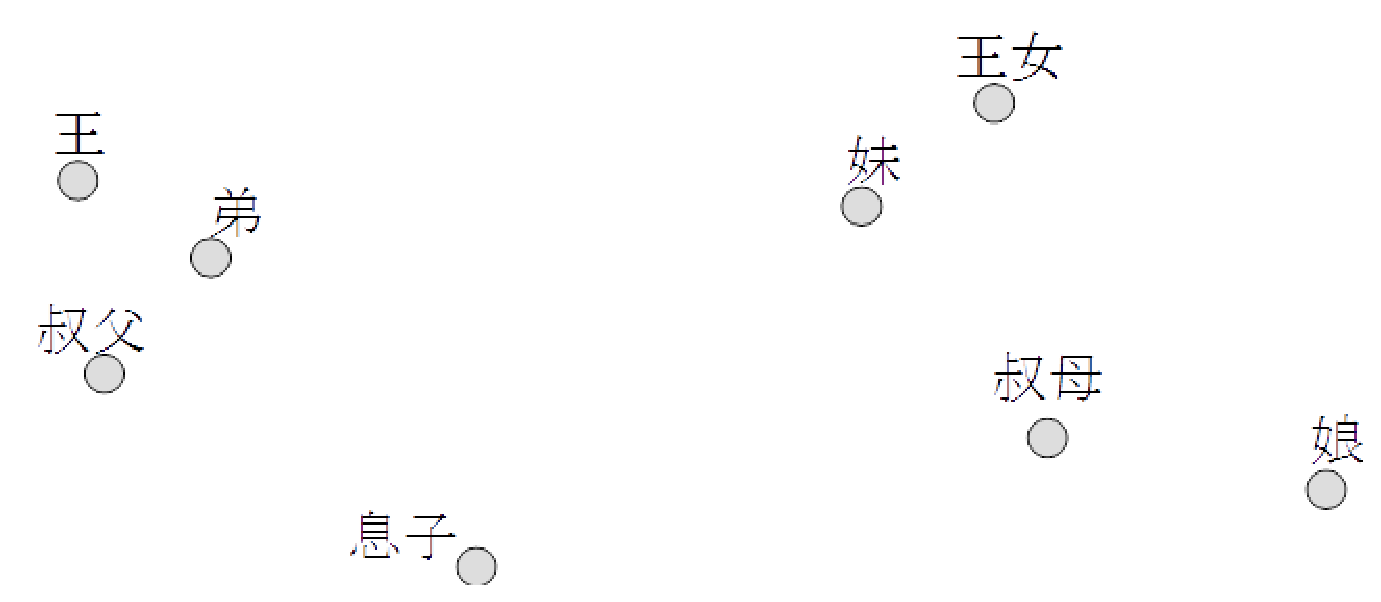
\includegraphics[width=8cm]{../images/kq_fv.eps}
  \caption{王-女王 近傍イメージ}
  \label{kq_fv}
\end{figure}

\begin{table}[h]
  \begin{minipage}[t]{.33\textwidth}
    \caption[(明るい,暗い)]{(明るい,暗い)の近傍単語}
    \begin{center}
      \begin{tabular}{|c|c|} \hline
        暗い & 明るい \\ \hline
        明るく & 暗く \\
        暗く & 明るく \\
        濃い & 薄暗い \\
        淡い & 眩しく \\
        眩しく & 青白い \\
        青白い & 濃い \\
        淡く & 薄暗く \\
        明るめ & 淡い \\
        鮮やか & ぼんやり \\ \hline
      \end{tabular}
    \end{center}
  \end{minipage}
  \begin{minipage}[t]{.66\textwidth}
    \caption[(光,影,闇)]{(光,影,闇)の近傍単語}
    \begin{center}
      \begin{tabular}{|c|c|c|} \hline
        太陽光 & 影の & 暗黒 \\ \hline
        反射 & 闇 & 妖魔 \\
        発光 & 暗闇 & 魔物 \\
        光線 & 暗部 & 邪悪 \\
        鏡 & 影 & 魔神 \\
        光源 & 暗い & 影 \\
        紫外線 & 隠れ & 悪魔 \\
        い光 & 暗黒 & 魔王 \\
        透かす & 其面 & 魔界 \\
        太陽 & 潜む & 魔 \\ \hline
      \end{tabular}
    \end{center}
  \end{minipage}
\end{table}
以上の結果を見るに、単純に近傍単語を同数取ってきたグループで作成するグラフは、与えた単語対が持つ関係を保持した同型のグラフには必ずしもなっていないことが予想される。
